\documentclass[xcolor=table,hyperref={pdfpagemode=FullScreen}]{beamer}
% struktūrizuojame, kad tas pats dokumentas tiktų ir konspektams ir skaidrėms
% Todėl \documentclass yra pašalinti
%xcolor=svgnames,
%xcolor=table
\beamertemplatenavigationsymbolsempty

\usepackage[ruled,vlined]{algorithm2e}
\DeclareMathOperator{\MinimalPoly}{\bf MinimalPoly}


%\setbeamercolor{section in head/foot}{fg=white,bg=black}






%\defbeamertemplate*{footline}{infolines theme}
%{
%  \leavevmode%
%  \hbox{%
%  \begin{beamercolorbox}[wd=.333333\paperwidth,ht=2.25ex,dp=1ex,center]{author in head/foot}%
%    \usebeamerfont{author in head/foot}\insertshortauthor
%  \end{beamercolorbox}%
%  \begin{beamercolorbox}[wd=.333333\paperwidth,ht=2.25ex,dp=1ex,center]{title in head/foot}%
%    \usebeamerfont{title in head/foot}\insertshorttitle
%  \end{beamercolorbox}%
%  \begin{beamercolorbox}[wd=.333333\paperwidth,ht=2.25ex,dp=1ex,right]{date in head/foot}%
%    \usebeamerfont{date in head/foot}\insertshortdate{}\hspace*{2em}
%    \insertframenumber{} / \inserttotalframenumber\hspace*{2ex}\hspace*{2em}
%  \end{beamercolorbox}%
%\begin{beamercolorbox}[ht=2.25ex,dp=3.75ex]{section in head/foot}
%\insertnavigation{\paperwidth}
%\end{beamercolorbox}%
%}%
%\vskip0pt%
%}

% slide number in right end of slide
\addtobeamertemplate{navigation symbols}{}{%
    \usebeamerfont{footline}%
    \usebeamercolor[fg]{footline}%
    \hspace{1em}%
    \vspace{-1em}%
    \insertframenumber/\inserttotalframenumber
}


\mode<presentation>
\usepackage{pgf}
\pgfdeclareimage[height=1cm]{image}{file}
\setbeamercolor{title}{fg=red!80!black, bg=red!20!white}
\setbeamertemplate{background canvas}[vertical shading][bottom=red!10,top=blue!10]
\useinnertheme[shadow=true]{rounded}
\useoutertheme{shadow}
\usecolortheme{orchid}
\setbeamerfont{block title}{size={}}
%\setbeamercolor{section in head/foot}{fg=red!10,bg=blue!10}
%\setbeamercolor{section in head/foot}{fg=white,bg=black}
%\setbeamertemplate{headline}{%
%   \begin{beamercolorbox}[ht=2.25ex,dp=3.75ex]{section in head/foot}
%        \insertnavigation{\paperwidth}
%    \end{beamercolorbox}%
%}%
%\mode<presentation>


%\makeatletter
%\setbeamertemplate{headline}{%
%    \begin{beamercolorbox}[ht=2.25ex,dp=3.75ex]{section in head/foot}
%        \insertnavigation{\paperwidth}
%    \end{beamercolorbox}%
%}%
%\makeatother





%\setbeamercovered{transparent}
\setbeamercovered{dynamic}




%\usetheme{progressbar}
%(or \usecolortheme{progressbar}, \usefonttheme{progressbar}, \useoutertheme{progressbar}, \useinnertheme{progressbar})


% Tiek skaidrėms tiek konspektams naudojami paketai

% svarbiausi paketai
\usepackage{amssymb}
\usepackage{amsmath}
\usepackage{graphicx}

% extended math fonts
\usepackage{yhmath}
\usepackage{url}
\usepackage[]{algorithm2e}
\usepackage{algpseudocode}


\DeclareMathOperator\arctanh{arctanh}
\DeclareMathOperator{\arcsinh}{arcsinh}


%\usepackage[authoryear]{natbib}

\bibliographystyle{apalike}
%\bibliographystyle{plainnat}
%\setcitestyle{square,aysep={}}

%\DeclareGraphicsExtensions{ps,eps,pdf}
\graphicspath{{figures/}}
%\usepackage[unicode]{hyperref}

% diagonal lines in tabulars
\usepackage{makecell}
\newcolumntype{x}[1]{>{\centering\arraybackslash}p{#1}}
\usepackage{tikz}
\newcommand\diag[4]{%
  \multicolumn{1}{p{#2}}{\hskip-\tabcolsep
  $\vcenter{\begin{tikzpicture}[baseline=0,anchor=south west,inner sep=#1]
  \path[use as bounding box] (0,0) rectangle (#2+2\tabcolsep,\baselineskip);
  \node[minimum width={#2+2\tabcolsep-\pgflinewidth},
        minimum  height=\baselineskip+\extrarowheight-\pgflinewidth] (box) {};
  \draw[line cap=round] (box.north west) -- (box.south east);
  \node[anchor=south west] at (box.south west) {#3};
  \node[anchor=north east] at (box.north east) {#4};
 \end{tikzpicture}}$\hskip-\tabcolsep}}





%lietuviskos raides

%\usepackage[latin1]{inputenc}
%\usepackage[utf8]{inputenc}
%\usepackage{fourier}
%\usepackage{times}
%\usepackage[T1]{fontenc}
%\usepackage[QX]{fontenc}

%\usepackage[L7x]{fontenc}
%\usepackage{lmodern}

%\usepackage[latin7]{inputenc}
%\usepackage{textcomp}

%\usepackage[lithuanian]{babel}
%\usepackage{hyperref}


%\input /usr/local/texlive/2007/texmf-dist/tex/plain/amsfonts/cyracc.def

%\input /usr/share/texmf/tex/plain/amsfonts/cyracc.def

%\font\tencyr=wncyr10 at 10pt
%\def\cyr{\tencyr\cyracc}
%\font\tencyrbib=wncyr10 at 9pt
%\def\cyrbib{\tencyrbib\cyracc}
%\font\tencyrit=wncyi10 at 10pt
%\def\cyrit{\tencyrit\cyracc}
%\font\tencyritbib=wncyi10 at 9pt
%\def\cyritbib{\tencyritbib\cyracc}
%\font\tencyrbf=wncyb10 at 10pt
%\def\cyrbf{\tencyrbf\cyracc}
%\font\tencyrbfbib=wncyb10 at 10pt
%def\cyrbfbib{\tencyrbfbib\cyracc}

% pataisymai del neaiskaus paketu susipjovimo raidems i kratkaja ir jo \"e

%\def\cyri{\hbox{\accent"24 i}}
%\def\cyre{\hbox{\accent"20 e}}
%\def\cyrI{\hbox{\accent"24 I}}
%\def\cyrE{\hbox{\accent"20 E}}
\newcommand{\ii}{\mathrm{i}} %imaginary unit
\newcommand{\ee}{\mathrm{e}} %exponent
\newcommand{\dd}{\mathrm{d}} %differential
\newcommand{\cl}[2]{\ensuremath{\mathit{Cl}_{#1,#2}}} % clifford algebra notation
% Quaternion base vectors
%\newcommand{\ii}{\mathrm{i}}
\newcommand{\jj}{\mathrm{j}}
\newcommand{\kk}{\mathrm{k}}


\def\d{\!\cdot\!} %narrow dot product
\def\w{\!\wedge\!} %narrow wedge product
\def\D{\cdot} %wide dot product
\def\W{\wedge} %wide wedge product


\newcommand{\e}[1]{\mathbf{e}_{#1}} % Clifford basis vectors in Cl(3,1)
\newcommand{\Ie}[1]{I\negthinspace\mathbf{e}_{#1}}%bivector in Cl(3,1)
\newcommand{\inv}[1]{\overline{#1}} %space inversion

\def\sR{\mathsf{R}} %sans serif Rotation
\def\sH{\mathsf{H}} %sans serif Hamiltonian
\def\sF{\mathsf{F}} %sans serif F
\def\sG{\mathsf{G}} %sans serif G

\newcommand{\bbR}{\ensuremath{\mathbb{R}}}
\newcommand{\bbP}{\ensuremath{\mathbb{P}}}
\newcommand{\bbC}{\ensuremath{\mathbb{C}}}
\newcommand{\bbH}{\ensuremath{\mathbb{H}}}
\newcommand{\bbF}{\ensuremath{\mathbb{F}}}


\def\m#1{\mathsf{#1}} % general multivector
\newcommand{\reverse}[1]{\widetilde{#1}}
\newcommand{\gradeinverse}[1]{\wideparen{#1}}
\newcommand{\cliffordconjugate}[1]{\wideparen{\widetilde{#1}}}

% General multivectors
\def\A{\mathsf{A}}
\def\B{\mathsf{B}}
\def\C{\mathsf{C}}
\def\D{\mathsf{D}}
\def\X{\mathsf{X}}
\def\m#1{\mathsf{#1}}%general multivector Input: $\m{a}$


% vectors = bold lower case
\newcommand{\ba}{\ensuremath{\mathbf{a}}}
\newcommand{\bb}{\ensuremath{\mathbf{b}}}
\newcommand{\bc}{\ensuremath{\mathbf{c}}}
\newcommand{\bd}{\ensuremath{\mathbf{d}}}
\newcommand{\be}{\ensuremath{\mathbf{e}}}
\newcommand{\bv}{\ensuremath{\mathbf{v}}}
\newcommand{\bV}{\ensuremath{\mathbf{V}}}
\newcommand{\bq}{\ensuremath{\mathbf{q}}}
\newcommand{\bu}{\ensuremath{\mathbf{u}}}


% bivectors = calligraphic
\newcommand{\cA}{\ensuremath{\mathcal{A}}}
\newcommand{\cB}{\ensuremath{\mathcal{B}}}
\newcommand{\cC}{\ensuremath{\mathcal{C}}}
\newcommand{\cU}{\ensuremath{\mathcal{U}}}

\DeclareMathOperator{\Det}{Det} %use Det for determinant of MV and \det for determinant of linear transformation
\newcommand{\magnitude}[1]{\lvert #1\rvert}
%amsbok stiliaus pakeitimai lietuviškai numeracijai
%\usepackage{mydefs}
%sutrumpinimai
%\input mydef.tex






% Nustatymai konspektų stiliui
\mode<article>
{
 \usepackage{fullpage}
 \usepackage{pgf}
 \usepackage{url}
}

\newcommand{\red}[1]{\textcolor{red}{#1}}
\newcommand{\blue}[1]{\textcolor{blue}{#1}}
\newcommand{\magenta}[1]{\textcolor{magenta}{#1}}
\definecolor{armygreen}{rgb}{0.29, 0.33, 0.13}
\definecolor{ao(english)}{rgb}{0.0, 0.5, 0.0}
\newcommand{\green}[1]{\textcolor{ao(english)}{#1}}
\newcommand{\mycomment}[1]{} % comment large piece of text



% boxed equations
\usepackage[most]{tcolorbox}

\tcbset{colback=yellow!10!white, colframe=red!50!black, 
        highlight math style= {enhanced, %<-- needed for the ’remember’ options
            colframe=red,colback=red!10!white,boxsep=0pt}
        }




% Nustatymai projektoriaus stiliui


%\setbeamerfont{title}{size=\tiny, parent=structure}
%\beamertemplatenavigationsymbolsempty
%\setbeamerfont{title}{family=\rmfamily}



%\mode<presentation>
%{
%  \setbeamertemplate{background canvas}[vertical shading][bottom=red!10,top=blue!10]
%  \usetheme{Marburg}
%   \usetheme{Warsaw}
%  \usefonttheme[onlysmall]{structurebold}
%  \usecolortheme[named=Teal]{structure}
%}




%{\usebeamercolor{palette primary}}



%\usetheme{Madrid}

%\setbeamercolor{section in head/foot}{fg=white,bg=black}

%\makeatletter
%\setbeamertemplate{headline}{%
%    \begin{beamercolorbox}[ht=2.25ex,dp=3.75ex]{section in head/foot}
%        \insertnavigation{\paperwidth}
%    \end{beamercolorbox}%
%}%
%\makeatother



%Titulinis puslapis
\title{Functions of multivector (MV): defective MV case
}
\author{A.~Acus$^{*}$ and A.~Dargys$^{**}$\\
\normalsize Vilnius University, Institute of Theoretical Physics
and Astronomy, Vilnius,
Lithuania\\
\normalsize $^{**}$Center for Physical and Technological Sciences
(CPTS), Vilnius, Lithuania
}



\title[Functions of MV: defective case]{Functions of multivector (MV): defective MV case}

\author[]{\underline{A.~Acus$^{*}$} and A.~Dargys$^{**}$}

\institute{${}^{*}$Vilnius University, Institute of Theoretical Physics
and Astronomy, Vilnius,
Lithuania\newline\noindent
$^{**}$Center for Physical and Technological Sciences
(CPTS), Vilnius, Lithuania
}

\date{December 12, 2024 }


\AtBeginSection[]
{
  \begin{frame}<beamer>
    \tableofcontents[currentsection,currentsubsection]
  \end{frame}
}

\colorlet{redshaded}{red!25!bg}
\colorlet{shaded}{black!25!bg}
\colorlet{shadedshaded}{black!10!bg}
\colorlet{blackshaded}{black!40!bg}

\colorlet{darkred}{red!80!black}
\colorlet{darkblue}{blue!80!black}
\colorlet{darkgreen}{green!80!black}

\def\radius{0.96cm}
\def\innerradius{0.85cm}

\def\softness{0.4}
\definecolor{softred}{rgb}{1,\softness,\softness}
\definecolor{softgreen}{rgb}{\softness,1,\softness}
\definecolor{softblue}{rgb}{\softness,\softness,1}

\definecolor{softrg}{rgb}{1,1,\softness}
\definecolor{softrb}{rgb}{1,\softness,1}
\definecolor{softgb}{rgb}{\softness,1,1}


\setbeamertemplate{headline}{%
\leavevmode%
  \hbox{%
    \begin{beamercolorbox}[wd=\paperwidth,ht=2.5ex,dp=1.125ex]{palette quaternary}%
    \insertsectionnavigationhorizontal{\paperwidth}{}{\hskip0pt plus1filll}
    \end{beamercolorbox}%
  }
}

%\useoutertheme[footline=authortitle]{miniframes}


%-----------


\begin{document}

\mycomment{
%%%%%%%%%%%%%%%%%%%%%%%%%%%%%%%%%%%%%%%%%%%%%%%%%
\foilhead{\color{MyBlue}Conclusions from numerical experiments}
}






{
\setbeamertemplate{headline}{}
\begin{frame}
  \titlepage
\end{frame}
}
%---------------------------------------------------------------------------------------------
\lecture{}{}
\author[ENGAGE Workshop \@ CGI 22, Sept 12]{A.~Acus and A.~Dargys}

%----      1   ------------------------------------

\section[Introduction;]{Introduction}
\begin{frame}
  \frametitle<presentation>{Notations and general properties}
\vskip -20pt
\begin{columns}[t]
\begin{column}{1.05\textwidth}
\begin{block}{Main results}
\begin{itemize}
  \item[1.] General \red{explicit} formula for exponential of multivector (MV) $\m{A}$ for \red{arbitrary $n=p+q$} expressed in terms of roots of characteristic equation is provided. \\[-40pt]
  \item[2.] The \red{implementation} is illustrated  by concrete examples.
  \item[3.] Straightforward adaptation of the obtained  formula allows to \red{compute any function} of MV.
\end{itemize}
\end{block}
\begin{block}{Defining property MV exponential}
\begin{equation*}
\left.\frac{\partial\exp(\m{A}t)}{\partial t}\right|_{t=1} = \m{A}
\exp(\m{A})=\exp(\m{A}) \m{A},\qquad \exp(0)=1\,.
\end{equation*} 
  The MV  $\m{A}$ is  \red{independent} of $t\in\bbR$. Since the MV
 always commutes with itself the multiplications from left and right by $\m{A}$ coincide.
  This  \red{can be applied in a proof} of  validity of  the exponential formulae   we have obtained.
\end{block}
\end{column}
\end{columns}
\end{frame}


% ------ 2---------
\begin{frame}
  \frametitle<presentation>{Notations and general properties}
\vskip -20pt
\begin{columns}[t]
\begin{column}{1.05\textwidth}
\begin{block}{Main involutions in real geometric algebras (GAs) $\cl{p}{q}$}
For a general MV that belongs to  $\cl{3}{0}$,
$n=p+q= 3$,
\begin{equation*}
\A=\,a_0+\underbrace{a_1\mathbf{e}_1+a_2\e{2}+a_3\e{3}}_{vector\
\ba}+
\underbrace{a_{12}\e{12}+a_{23}\e{23}+a_{13}\e{13}}_{bivector\
\cA}+a_{123}I
\end{equation*}
\begin{align*}
  &\reverse{\m{A}}=a_0+\ba-\cA-a_{123}I,&&\quad\text{reversion}\\
  &\gradeinverse{\m{A}}=a_0-\ba+\cA-a_{123}I,&&\quad\text{grade inversion}\\
  &\cliffordconjugate{\m{A}}=a_0-\ba-\cA+a_{123},I&&\quad\text{Clifford
conjugation}\\
  &\overline{\m{A}}=a_0-\ba-\cA-a_{123}I=2\langle\m{A}\rangle_{0}-\m{A},&&\quad\text{nonscalar part negation}
\end{align*}
\end{block}
\begin{block}{Involution properties  of  the exponential}
\begin{equation*}
\reverse{\ee^{\m{A}}}=\ee^{\reverse{\m{A}}},\qquad\gradeinverse{\ee^{\m{A}}}=\ee^{\gradeinverse{\m{A}}},
\qquad \cliffordconjugate{\ee^{\m{A}}}=\ee^{\cliffordconjugate{\m{A}}},
  \qquad \overline{\ee^{\m{A}}}=\ee^{\overline{\m{A}}}\,.
\end{equation*}
\end{block}
\end{column}
\end{columns}
\end{frame}


% ------ 3 ---------
\begin{frame}
  \frametitle<presentation>{General properties of GA exponential}
\vskip -20pt
\begin{columns}[t]
\begin{column}{1.05\textwidth}
\begin{block}{Series expansions}
 P.~Lounesto, {\em Clifford Algebra and Spinors},
1997.
\abovedisplayskip=8pt
\belowdisplayskip=8pt
\begin{equation*}
  \begin{split}
  \ee^{\m{A}}=&1+\frac{\m{A}}{1!}+\frac{\m{A}^2}{2!}+\frac{\m{A}^3}{3!}+\frac{\m{A}^4}{4!}+\dots,
\end{split}
\end{equation*}
  Convergence radius is \red{infinite}. Convergence is \red{not monotonic}: coefficients may acquire \red{very large values} before starting to converge. 
\end{block}
\vskip -5pt
\begin{block}{Numerical experiment with \cl{3}{0}}
$\red{\m{A}=-8-6\e{2}-9\e{3}+5\e{12}-5\e{13}+6\e{23}-4\e{123}};\qquad a_{12}=5$
  \end{block}
\end{column}
\end{columns}
\begin{columns}[t]
\begin{column}{0.45\textwidth}
\begin{flushleft}
\vspace{-73pt}
\includegraphics[width=5cm,trim=0cm 0cm 0cm 0cm]{fig1.eps}
\end{flushleft}
\end{column}\qquad 
\begin{column}{0.75\textwidth}
\parbox[r][.4\textheight][t]{0.81\textwidth}{
Alternating bell-like convergence. Dependence of
coefficient $a_{12}$ on a number of terms in GA
exponential series. $20$ terms give $a_{12}=0.902645\times 10^6$.
$70$ terms give $a_{12}=-1.64146$ which is close to exact value. Similar
  behavior is observed for other coefficients.
}
\end{column}
\end{columns}
\end{frame}



%--4----------------
\section[Characteristic coefficients;]{Characteristic equation in GA  and coefficient  properties}
\begin{frame}
\frametitle<presentation>{Characteristic coefficients}
\vskip -0pt
\begin{columns}[t]
\begin{column}{1.05\textwidth}
\begin{block}{Degree of characteristic polynomial}
  Every MV $\m{A}\in\cl{p}{q}$ has a \red{characteristic polynomial}
\abovedisplayskip=6pt
\belowdisplayskip=6pt
\begin{equation*}\label{CharPolyDef}
  \chi_{\m{A}}(\lambda)=-\Det(\lambda -\m{A})=\sum_{k=0}^{d} C_{(d-k)}(\m{A})\, \lambda ^k.
\end{equation*}
of degree $d$, where
$d=2^{\lceil\tfrac{n}{2}\rceil}$ is the integer, $n=p+q$. In
particular, $d=2^{n/2}$ if $n$ is even and $d=2^{(n+1)/2}$ if $n$
is odd. \red{The integer $d$  may be interpreted as a dimension of
real or complex matrix representation of a considered GA} in the
8-fold Bott periodicity table.\newline 

\small
The coefficients $C_{(m)}(\m{A})$  depend on a selected GA and  MV $\m{A}$. At the
highest power of  $\lambda$ we assume $C_{(0)}=-1$. The
  coefficient $C_{(1)}(\m{A})$ represents \red{MV trace},
  $C_{(1)}(\m{A})=\mathop{\mathrm{Tr}}(\m{A})=d \left\langle\m{A}\right\rangle_{0}$,
where $\left\langle\m{A}\right\rangle_{0}$ is the scalar
  part of MV. The coefficient $C_{(d)}(\m{A})$ is related to \red{MV
  determinant} $\Det\m{A}=-C_{(d)}(\m{A})$.
\end{block}
\end{column}
\end{columns}
\end{frame}


%--5---------------- 
\begin{frame}
\frametitle<presentation>{Methods to find characteristic coefficients in GA}
\vskip -18pt
\begin{columns}[t]
\begin{column}{1.10\textwidth}
  \begin{block}{Optimized $\Det(\m{A})$ formulas for low dimension algebras, $n\le 6$}
 \begin{table}
\begin{center}
  \begin{tabular}{cc}
    $\cl{p}{q}$& $\Det(\m{A})$ \\\hline
\rule{0pt}{3ex}
$p+q=1,2$&$\m{A}\bar{\m{A}}$\\
$p+q=3,4$ &$
    \frac{1}{3}\bigl(\m{A}\m{A} \overline{\m{A}\m{A}}+2 \m{A}\overline{\bar{\m{A}}\overline{\bar{\m{A}}\bar{\m{A}}}} \bigr)$
\\
$n=p+q=5,6$ &$
    \frac{1}{3}\bigl(\m{H}\m{H} \overline{\m{H}\m{H}}+2 \m{H}\overline{\bar{\m{H}}\overline{\bar{\m{H}}\bar{\m{H}}}} \bigr)\qquad\textrm{with}\quad \m{H}=\m{A}\reverse{\m{A}}$
\end{tabular}
\end{center}
\end{table}
   In the Table there are given  \red{optimized formulae}   to calculate the GA determinant. 
   To get values of \red{remaining} 
   $C_{(k)}(\m{A})$ of characteristic  
  polynomial, it is enough to replace $\Det(\m{A})$ by function 
   $\Det(\lambda-\m{A})$. 
 For example, taking $\m{A}=-4-\e{1}-\e{2}-\e{3}-\e{4}-2 \sqrt{3} \e{1234}$ of $\cl{4}{0}$ we obtain 
\abovedisplayskip=10pt
\belowdisplayskip=8pt
 \begin{equation*}
 \begin{split}
   \chi_{\m{A}}(\lambda)&=C_{(4)}(\m{A})+C_{(3)}(\m{A})
\lambda+C_{(2)}(\m{A})\lambda^2+C_{(1)}(\m{A})
   \lambda^3+C_{(0)}(\m{A})\lambda^4\\
   &
 = -64 \lambda^2-16 \lambda^3-\lambda^4,
\end{split}
 \end{equation*}
    i.e. $C_{(0)}=-1$, $C_{(1)}=-16$, $C_{(2)}=-64$, $C_{(3)}=0$, $C_{(4)}=0$.
\end{block}
\end{column}
\end{columns}
\end{frame}



%--6---------------- 
\begin{frame}
\frametitle<presentation>{Characteristic coefficients}
\vskip -16pt
\begin{columns}[t]
\begin{column}{1.08\textwidth}
  \begin{block}{Faddeev-Leverrier method}
In Faddeev-Leverrier method~\cite{Householder1975,Hou1998,Shirokov2021,Helmstetter2019}
the coefficients $C_{(k)}(\m{A})$ of char. 
    polynomial are calculated \red{recursively},
beginning from $C_{(1)}(\m{A})$ and ending with $C_{(d)}(\m{A})$. We
start from multivector $\m{A}_{(1)}$ by setting
$\m{A}_{(1)}=\m{A}$. Then  we compute the coefficient
$C_{(k)}(\m{A})=\frac{d}{k}\langle \m{A}_{(k)} \rangle_{0}$ , where $\langle \m{A}_{(k)} \rangle_{0}$ is the scalar part, and in
the next step the new MV $\m{A}_{(k+1)}=\m{A}
\bigl(\m{A}_{(k)}-C_{(k)}\bigr)$:
\abovedisplayskip=12pt
\belowdisplayskip=12pt
\begin{equation*}\label{FLAlg}
  \begin{array}{rcl}
 \m{A}_{(1)}=\m{A}&\rightarrow&C_{(1)}(\m{A})=\frac{d}{1}\langle \m{A}_{(1)}\rangle_0,\\
   % &\swarrow&\\[-3pt]
 \m{A}_{(2)}=\m{A}\bigl(\m{A}_{(1)}-C_{(1)}\bigr)
&\rightarrow&C_{(2)}(\m{A})=\frac{d}{2}\langle \m{A}_{(2)}\rangle_0,\\
    &\vdots&\\
 \m{A}_{(d)}=\m{A}\bigl(\m{A}_{(d-1)}-C_{(d-1)}\bigr)
&\rightarrow&C_{(d)}(\m{A})=\frac{d}{d}\langle
\m{A}_{(d-1)}\rangle_0.
\end{array}
\end{equation*}
    The \red{determinant} of MV then is
\abovedisplayskip=6pt
\begin{equation*}
  \Det(\m{A})=\m{A}_{(d)}=-C_{(d)}=\m{A}
\bigl(\m{A}_{(d-1)}-C_{(d-1)}\bigr)\,.\end{equation*}
\end{block}
\end{column}
\end{columns}
\end{frame}


%--7---------------- 
\begin{frame}
\frametitle<presentation>{Characteristic coefficients}
\vskip -16pt
\begin{columns}[t]
\begin{column}{1.05\textwidth}
  \begin{block}{Other properties of characteristic polynomials}
The coefficients of char. polynomial and  equation  $\chi_{t\m{A}}(\lambda)=0$ satisfy the following
properties
\begin{align}\label{propertyDC}
  \frac{\partial C_{(k)}(t \m{A})}{\partial t}=k t^{k-1}  C_{(k)}(t \m{A}),\qquad
  \frac{\partial C_{(1)}(t \m{A}^k)}{\partial t}&=k t^{k-1}  C_{(1)}(t \m{A}^k),
\end{align}
where $t$ is a scalar parameter. We  need
the above properties in  proof of \red{main theorem} below,  which   states that  GA exponential
can be expressed by the  roots $\lambda_i$ of characteristic equation and a finite product of MVs due to Cayley-Hamilton theorem
applied to Clifford algebra \cl{p}{q}.
\end{block}
\end{column}
\end{columns}
\end{frame}


%--8---------------- 
\section[Exponential of MV;]{Exponential of general MV}
\begin{frame}
\frametitle<presentation>{Main result (theorem)}
\vskip -19pt
\begin{columns}[t]
\begin{column}{1.15\textwidth}
\begin{theorem}[MV exponential in basis-free form]
  In $\cl{p}{q}$ the exponential of a \red{general multivector} $\m{A}$ can be computed as
  \begin{align}&\notag\\[-25pt]
\mkern-0mu \red{\exp(\m{A})}
  &=\tcboxmath{\sum_{i=1}^{d} \ee^{\lambda_i}\,\beta(\lambda_i)
    \sum_{m=0}^{d-1} \biggl(\sum_{k=0}^{d-m-1}\lambda_i^k C_{(d-k-m-1)}(\m{A})\biggr)\, \m{A}^{m}}\label{expNcomplexCoordFree}
  \\
  &= \sum_{i=1}^{d} \ee^{\lambda_i}\Bigl(\frac{1}{d}+\beta(\lambda_i)\m{B}(\lambda_i)\Bigr),\quad
  \beta(\lambda_i)={ \frac{1}{\sum_{j=0}^{d-1}(j+1)\,C_{(d -j-1)}(\m{A})\, \lambda_i^{j}}}\notag \\
  &\mathrm{where}\quad\m{B}(\lambda_i)=  \sum_{m=0}^{d-2} \biggl(\sum_{k=0}^{d-m-2}\lambda_i^k C_{(d-k-m-2)}(\m{A})\biggr)\, \langle\m{A}^{m+1}\rangle_{-0}\,. \notag 
\end{align}
The last symbol
$\langle\m{A}^{m+1}\rangle_{-0}\equiv\frac{1}{2}\bigl(\m{A}^{m+1}-\overline{\m{A}^{m+1}}\bigr)$
indicates that all grades of multivector $\m{A}^{m+1}$ are
included except grade-$0$,
  because
the scalar part is simply a sum of exponents of eigenvalues divided by $d$.
\end{theorem}
\end{column}
\end{columns}
\end{frame}



%--9----------------
\begin{frame}
\frametitle<presentation>{Proof of theorem}
\vskip -19pt
\begin{columns}[t]
\begin{column}{1.15\textwidth}
  \begin{block}{Sketch of proof}
    It is enough to \red{check the defining equation}
\begin{equation*}
\left.\frac{\partial\exp(\m{A}t)}{\partial t}\right|_{t=1} = \m{A}
\exp(\m{A})=\exp(\m{A}) \m{A}. 
\end{equation*} 
First, using properties of characteristic coefficients
\eqref{propertyDC} and noting that replacement $\m{A}\to\m{A}t$
implies $\lambda_i\to \lambda_i t$ and then performing differentiation
$\left.\frac{\partial\exp(\m{A}t)}{\partial t}\right|_{t=1}$ we
obtain that $\exp(\lambda_i)$  of right hand side of
\eqref{expNcomplexCoordFree} is replaced by
$\lambda_i\exp(\lambda_i)$,
\begin{align*}
  \left.\frac{\partial\exp(\m{A}t)}{\partial t}\right|_{t=1}=&\sum_{i=1}^{d} \blue{\lambda_i}\exp(\lambda_i)\beta(\lambda_i)\,
  \sum_{m=0}^{d-1} \biggl(\sum_{k=0}^{d-m-1}\lambda_i^k C_{(d-k-m-1)}(\m{A})\biggr)\, \m{A}^{m},
\end{align*}
where the weight factor $\beta(\lambda_i)$ plays no role in
the proof. 
\end{block}
\end{column}
\end{columns}
\end{frame}

%--10 ----------------
\begin{frame}
\frametitle<presentation>{Proof of theorem}
\vskip -19pt
\begin{columns}[t]
\begin{column}{1.15\textwidth}
  \begin{block}{Sketch of proof (continuation I)}
     Next, multiply basis-free formula
\eqref{expNcomplexCoordFree} by $\m{A}$
\begin{align*}
\m{A}\exp(\m{A})=\sum_{i=1}^{d} \exp(\lambda_i)\,\beta(\lambda_i)
  \sum_{m=0}^{d-1} \biggl(\sum_{k=0}^{d-m-1}\lambda_i^k C_{(d-k-m-1)}(\m{A})\biggr)\, \m{A}^{\blue{m+1}}\,,
\end{align*}
    and \red{subtract} the second equation from the first for \red{each fixed}
root $\lambda_i$, i.e. temporary ignore summation over roots, to get
\begin{align*}\label{difFormula}
  &\mkern-8mu  \left.\biggl(\left.\frac{\partial\exp(\m{A}t)}{\partial t}\right|_{t=1}\!\!- \m{A}\exp(\m{A})\biggr)\right|_{\lambda_i}
  \!\!=
  \ee^{\lambda_i}\, \beta(\lambda_i)
  \Bigl(
  \sum_{k=1}^{d} \lambda_i^k C_{(d-k)}(\m{A})-\m{A}^{k} C_{(d-k)}(\m{A})
  \Bigr)\notag\\
  &\qquad  =\exp(\lambda_i) \,\beta(\lambda_i)\Bigl(
  \bigr(\lambda_i^d -\m{A}^{d}\bigr) C_{(0)}(\m{A})+\cdots + \bigr(\lambda_i -\m{A}\bigr) C_{(d-1)}(\m{A})
  \Bigr)\,.
\end{align*}
\end{block}
\end{column}
\end{columns}
\end{frame}


%--11 ----------------
\begin{frame}
\label{proofLastSlide}
\frametitle<presentation>{Proof of theorem}
\vskip -19pt
\begin{columns}[t]
\begin{column}{1.05\textwidth}
  \begin{block}{Sketch of proof (continuation II)}
 Using Cayley-Hamilton \red{relation} for $\m{A}$, which follows from Faddeev-Leverrier algorithm in GA form,
\abovedisplayskip=5pt
\belowdisplayskip=5pt
\begin{align*}
  \sum_{k=0}^{d}  \m{A}^k C_{(d-k)}(\m{A})=\m{A}^{d}C_{(0)}(\m{A})+\m{A}^{d-1}C_{(1)}(\m{A})+\cdots + C_{(d)}(\m{A})= &0\notag,
\end{align*}
and  similar relation for $\lambda_i^d$, we solve for the highest
powers $\m{A}^{d}$ and $\lambda_i^d$, and  substitute them
into the difference formula. After expansion we
    obtain that the sum is equal to  zero for each possible $\lambda_i$.
\end{block}   
\begin{block}{Notes to the main theorem}
\begin{itemize}
\item Since \red{roots} can be \red{complex}, the result is \red{formally complex}.
\item We have obtained \red{basis-related formula} as well.
\item MV $\m{A}$ should be \red{diagonalizable}, i.e. 
  \hyperlink{MinimalPolynomial}{\beamerbutton{\large minimal polynomial}}, should not have multiple roots (for $ n> 2$).
\end{itemize}
\end{block}
\end{column}
\end{columns}
\end{frame}




%--12 ----------------
\begin{frame}
\frametitle<presentation>{Exponential of MV in \cl{4}{0} with multiple zero eigenvalue}
\vskip -10pt
\begin{columns}[t]
\begin{column}{1.05\textwidth}
 \begin{block}{Example of exponential of $\m{A}=-4-\e{1}-\e{2}-\e{3}-\e{4}-2 \sqrt{3} \e{1234}$}
  Using Table of optimized determinant formulas one can verify that \red{$\Det(\m{A})=0$}.
For algebra $\cl{4}{0}$ we find $d=4$. The characteristic
  polynomial is 
 \begin{equation*}
 \begin{split}
   \chi_{\m{A}}(\lambda)&=C_{(4)}(\m{A})+C_{(3)}(\m{A})
\lambda+C_{(2)}(\m{A})\lambda^2+C_{(1)}(\m{A})
   \lambda^3+C_{(0)}(\m{A})\lambda^4\\
   &
 = -64 \lambda^2-16 \lambda^3-\lambda^4 = -\lambda^2 (8+\lambda)^2.
 \end{split}
 \end{equation*}
The roots are $\lambda_1=0, \lambda_2=0, \lambda_3=-8, \lambda_4=-8$. Since multiple roots appear,  we have to compute \hyperlink{MinimalPolynomial}{\beamerbutton{\large minimal polynomial}}
 of $\m{A}$,
which is $\mu_{\m{A}}(\lambda)=\lambda (8 + \lambda)$. Since
minimal polynomial has only linear factors, i.e. the polynomial is square
  free, the \red{MV is diagonalizable}, and the formula for
$\mu_{\m{A}}(\lambda)$  can be applied without modification.
 \end{block}
\end{column}
\end{columns}
\end{frame}



%--13 ----------------
\begin{frame}
\frametitle<presentation>{Exponential of MV in \cl{4}{0} with multiple zero eigenvalue}
\vskip -10pt
\begin{columns}[t]
\begin{column}{1.05\textwidth}
  \begin{block}{Example of exponential (continuation I)}
 Then we have
\begin{equation*}\label{example3Bi}
\begin{split}
  \beta(\lambda_i)\m{B}&(\lambda_i)= \scriptstyle\frac{1}{\sum_{j=0}^{d-1}(j+1)\,C_{(d -j-1)}(\m{A})\, \lambda_i^{j}}
  \sum_{m=0}^{d-2} \sum_{k=0}^{d-m-2}\!\!\!\lambda_i^k C_{(d-k-m-2)}(\m{A})\, \langle\m{A}^{m+1}\rangle_{-0}\\[3pt]
  =&\textstyle
 \frac{8+\lambda_i}{4 \lambda_i (4+\lambda_i)}\langle\m{A}\rangle_{-0}+ \frac{16+\lambda_i}{4 \lambda_i (4+\lambda_i) (8+\lambda_i) }\langle\m{A}^{2}\rangle_{-0}+\frac{1}{4 \lambda_i (4+\lambda_i) (8+\lambda_i) }\langle\m{A}^{3}\rangle_{-0}
  \\
  =&\scriptstyle -\frac{1}{\lambda_i +4}-\frac{1}{4 (\lambda_i +4)}\e{1}-\frac{1}{4 (\lambda_i +4)}\e{2}-\frac{1}{4 (\lambda_i +4)}\e{3}-\frac{1}{4 (\lambda_i +4)}\e{4}-\frac{\sqrt{3}}{2 \lambda_i +8}\e{1234}\/.
\end{split}
\end{equation*}
    From the \red{middle line} one may suppose that the sum over
    roots would yield \red{division by zero} due to zero denominators. The
    \red{last line}, however, demonstrates that this is not the case, since
after collecting terms at basis elements we see that all potential
    \red{zeroes} in the denominators \red{have been cancelled}. Unfortunately the
    \red{cancellation does not occur for non-diagonalizable MVs}.
 \end{block}
\end{column}
\end{columns}
\end{frame}


%--14 ----------------
\begin{frame}
\frametitle<presentation>{Exponential of MV in \cl{4}{0} with multiple zero eigenvalue}
\vskip -10pt
\begin{columns}[t]
\begin{column}{1.05\textwidth}
  \begin{block}{Example of exponential (continuation II)}
 Lastly,
after performing summation $\sum_{i=1}^{d}
    \blue{\exp(\lambda_i)}\bigl(\frac{1}{d}+\beta(\lambda_i)\m{B}(\lambda_i)\bigr)$
over complete set of roots
$\{\lambda_1,\lambda_2,\lambda_3,\lambda_4\}=\{0,0,-8,-8\}$ with
    \red{exponent weight factor} $\exp(\lambda_i)$, which can be replaced by
any other function or transformation (see
below) we obtain
\abovedisplayskip=5pt
\belowdisplayskip=5pt
\begin{align*}
  \exp(\m{A})= & \frac{1+\ee^8}{2 \ee^8}+
\frac{1-\ee^8}{8 \ee^8}\big(\e{1}+ \e{2}+\e{3}+
   \e{4}-2\sqrt{3}\e{1234}\,\big).
\end{align*}
\end{block}
\begin{block}{Notes}
\begin{itemize}
  \item For exponential (and other real functions) the answer always can be made \red{real by summing pairwise complex roots}.
  \item It appears that the main theorem can applied to compute \red{any GA function $f(\m{A})$}  if root exponentials are replaced by $\blue{\exp(\lambda_i)\to f(\lambda_i)}$
\end{itemize}
\end{block}\end{column}
\end{columns}
\end{frame}


%--15 ----------------
\begin{frame}
\frametitle<presentation>{Exponential of MV}
\vskip -19pt
\begin{columns}[t]
\begin{column}{1.14\textwidth}
  \begin{block}{Making (exact) answer real }
%\scriptsize 
Exponential formula~\eqref{expNcomplexCoordFree}
includes summation over (in general complex) roots
    of characteristic polynomial. Formally the \red{result is a
    complex} number.
Denoting conjugate root pair as $\lambda_r\pm\ii\lambda_i$, and computing
    the \red{sum over a single complex conjugate root pair} we come to the
 relation
\begin{align*}\label{ccPair}
\textstyle 
  \ee^{\lambda_r + \ii\lambda_i}\, \frac{\m{C} + \ii\m{D}}{g + \ii h} + \ee^{\lambda_r - \ii\lambda_i}\, \frac{\m{C} - \ii\m{D}}{g - \ii h}=
  \frac{2 \ee^{\lambda_r} \bigl((g\,\m{C}+h\,\m{D}) \cos\lambda_i+(h\,\m{C}-g\,\m{D}) \sin\lambda_i\bigr)}{g^2+h^2},
\end{align*}
where $\m{C},\m{D}\in$\cl{p}{q} are real MV's and $g,h\in\bbR$.
    The right hand side of this equation now is \red{formally real MV}.
From symbolic computation point of view the issue is not
so simple.  In \textit{Mathematica} the formal solution is represented as
    \red{Root[poly,\,k]} (when $d\ge 5$ solutions are \red{not solvable in radicals}). To obtain real answer we have to manipulate these formal objects algebraically with \red{RootReduce[\,]} command, which produces another Root[poly$^\prime$,\,k$^\prime$] object. Root reduction
typically raises the order of the irreducible polynomial.
\end{block}\end{column}
\end{columns}
\end{frame}



\section[Other functions;]{Other elementary and special functions}
%--16----------------
\begin{frame}
\frametitle<presentation>{Functions of MV}
\vskip -15pt
\begin{columns}[t]
\begin{column}{1.05\textwidth}
  \begin{block}{Elementary functions} 
The main theorem~\eqref{expNcomplexCoordFree} is universal.
It allows to compute \red{any elementary GA function}
 if  the exponential weight $\blue{\exp(\lambda_i)}$ is replaced by any other function. 
For example, if in $\sum_{i=1}^{d} \ee^{\lambda_i}\Bigl(\frac{1}{d}+\beta(\lambda_i)\m{B}(\lambda_i)\Bigr)$   
$\ee^{\lambda_i}$ is replaced  by $\log(\lambda_i)$
we obtain the  logarithm of MV
\begin{equation*}\label{logfromexp}
\begin{split}
  \log{\m{A}}=&\frac{1}{2}(\log (0_{+})
  +\log (-8))\\
  &\quad+\frac{1}{8} (\log (-8)-\log (0_{+})) \left(\e{1}+\e{2}+\e{3}+\e{4}+2 \sqrt{3} \e{1234}\right).
\end{split}
 \end{equation*}
If we assume that $\exp\bigl(\log (0_{+})\bigr)=\lim_{x\to
0_{+}}\exp\bigl(\log (x)\bigr)=0$ and $\exp\bigl(\log
(-8)\bigr)=-8$, then it is easy to check that
under these assumptions the  exponentiation of $\log{\m{A}}$ 
    yields $\exp(\log(\m{A}))=\m{A}$, i.e., the $\log$ function is a \red{formal inverse} of $\exp$.
 \end{block}
\end{column}
\end{columns}
\end{frame}




%--17----------------
\begin{frame}
\frametitle<presentation>{Functions of MV}
\vskip -15pt
\begin{columns}[t]
\begin{column}{1.07\textwidth}
  \begin{block}{Trigonometric/hyperbolic and special functions} 
    In a similar way we can find \red{hyperbolic} and \red{trigonometric}
   GA  functions and their inverses (\red{complex
    numbers are inevitable in computing trigonometric} functions in the
    most of real Clifford algebras). After replacement of 
$\exp(\lambda_i)$ by  $\sinh(\lambda_i)$, $\arcsinh(\lambda_i)$ and Bessel $J_0(\m{A})$
in~\eqref{expNcomplexCoordFree} one finds, respectively,
\begin{equation*}
\begin{split}
  \sinh{\m{A}}=&\frac{1}{8}\sinh(8)\bigl(-4-\e{1}- \e{2}-\e{3}-\e{4}-2 \sqrt{3} \e{1234}\bigr),\\
  \arcsinh{\m{A}}=&\frac{1}{8}\arcsinh(8)\bigl(-4 -\e{1} - \e{2}-\e{3}-\e{4} -2 \sqrt{3} \e{1234} \bigr),\\
  J_0(\m{A})=& \frac{1}{2} (1+J_0(8))+
 \frac{1}{8} (J_0(8)-1) \bigl(\e{1}+\e{2}+\e{3}+\e{4}+2\sqrt{3} \e{1234} \bigr)
\end{split}
\end{equation*}
It is easy to check that $\sinh\bigl(\arcsinh(\m{A})\bigr)=\m{A}$
    is  satisfied indeed. \red{Special functions} of MV argument  can be computed in the same way.
 \end{block}
\end{column}
\end{columns}
\end{frame}

%\hyperlink{WhySquareOfMatrixFails}{\beamerbutton{"Why square roots of Bott matrices fail?"}}). 


\section[Conclusions and perspective]{Conclusions and perspective}

%--23----------------
\begin{frame}
\vspace{-20pt}
\begin{columns}[t]
\begin{column}{1.06\textwidth}
\begin{block}{Conclusions and perspective}
\begin{itemize}\small
  \item <1->  Algebraic formulas to compute GA exponentials in  $\cl{p}{q}$ real algebras
   in terms of MV char. equation roots have been found when the MV is  diagonalizable. 
 \item <2->  \red{Big surprise!} The presented formulas can be extended to compute arbitrary elementary and special functions of MV.
 \item <3->  Functions $f(\m{A})$ of non-diagonalizable MV $\m{A}$ can be computed after perturbation of initial MV
  (by adding small symbolic MV, for example, $\varepsilon\e{1}$), end then computing the limiting case
   $\lim_{\varepsilon\to 0} f(\m{A}+\varepsilon\e{1})$.
\end{itemize}
\end{block}

\begin{block}{Implementation} 
  \red{We have programmed} the described formulas (both in orthonormal basis and basis-free form) in {\it Mathematica} package, 
  which may be downloaded from 
  \blue{\url{https://github.com/ArturasAcus/GeometricAlgebra}}. 

\scriptsize Examples are provided in the notebook ElementaryFunctions.nb.
\end{block}
  \begin{flushright}\vskip -15pt  \Huge \blue{Thank You\hbox to 1.5cm{}}
\end{flushright}

\end{column}
\end{columns}
\end{frame}


%\end{document}

\begin{frame}
\vspace{-5pt}
\frametitle<presentation>{Bibliography\hfill }
\begin{thebibliography}{}
%\setlength{\textwidth}{14cm} 
\tiny

\bibitem{Fujii2012}
Fujii, K., Oike, H. 
\newblock    How to calculate the exponential of matrices.
    \newblock   \hbox{\hbox to 0.67cm{}Far East Journal of Mathematical Education  \textbf{9}(1),  39--55 (2012), p-ISSN:  0973-5631, arXiv:quant-ph/0604115v1}

\bibitem{Hou1998}
Shui-Hung, H. 
\newblock
    Classroom note: A simple proof of the {L}everrier-faddeev
  characteristic polynomial algorithm. 
\newblock    SIAM Review.  \textbf{40}(3),  706--709 (1998)

\bibitem{Chappell2015}
J.~M. Chappell, A.~Iqbal, L.~J. Gunn, and D.~Abbott,
\newblock Functions of multivector variables,
\newblock PLoS ONE {\bf 10}(3), 1--21 (2015),
%\newblock Doi:10.1371/journal.pone.0116943.

\bibitem{Householder1975}
Householder, A.S.
\newblock The Theory of Matrices in Numerical Analysis. 
\newblock  Dover Publications, Inc, New York, N. Y. 10014 (1975)


\bibitem{DargysAcus2021a}
A.~Dargys and A.~Acus,
\newblock Exponentials of general multivector (MV) in $n=3$ {C}lifford
  algebras,
\newblock Nonlinear Analysis: Modelling and Control , 3 (2021),
%\newblock submitted to \textit{Nonlinear Analysis: Modelling and Control}.

\bibitem{Shirokov2021}
D.~S. Shirokov,
\newblock On determinant, other characteristic polynomial coefficients, and
  inverses in Clifford algebras of arbitrary dimension,
\newblock Computational and Applied Mathematics  PLoS ONE {\bf 40}(5),(2021);  {\bf arXiv: 2005.04015}(2020).

\bibitem{Helmstetter2019}
Helmstetter, J.: 
\newblock Characteristic polynomials in clifford algebras and in more
  general algebras. 
\newblock Adv. Appl. Clifford Algebras  \textbf{29}(30) (2019)

\bibitem{AcusDargysPreprint2020}
A.~Acus and A.~Dargys,
\newblock Square root of a multivector of {C}lifford algebras in 3{D}: A game
  with signs,
\newblock arXiv:2003.06873 {\bf math-phi}, 1--29,
\end{thebibliography}
%\vskip 20pt
%\begin{center}
%\alert{\huge Thank You}
%\end{center}
\end{frame}

%--Appendix----------------
\begin{frame}
%\frametitle<presentation>{Functions of MV}
\vskip -15pt
\begin{columns}[t]
\begin{column}{1.07\textwidth}
\begin{block}{Minimal polynomial of MV\hyperlink{proofLastSlide}{\beamerbutton{Back to proof}}} 
  \begin{algorithm}[H]
\small
\SetAlgoLined \SetNoFillComment \LinesNotNumbered
\SetKwInput{KwInput}{Input}
\SetKwInput{KwOutput}{Output}
\SetKwProg{minimalPoly}{minimalPoly}{}{}$\MinimalPoly{(\m{A})}${\\
\KwInput{multivector $\m{A}=a_0+\sum_J^{2^n-1}a_J\e{J}$ and polynomial variable $x$}
\KwOutput{minimal polynomial $c_1+c_2 x+c_3 x^2+\cdots$}
  {\scriptsize \tcc{Initialization}}
nullSpace=\{\};\quad lastProduct=1;\quad vectorList=\{\}\;
  {\scriptsize\tcc{keep adding new MV coefficient vectors to vectorList until null space becomes nontrivial}}
  While[nullSpace===\{\},\\
  lastProduct=$\m{A}\circ$lastProduct\;
  AppendTo[vectorList,\, ToCoefficientList[lastProduct]]\;
  nullSpace=NullSpace[Transpose[vectorList]];\\
 \qquad ]\;
  {\scriptsize\tcc{use null space weights to construct the polynomial $c_1+c_2 \m{A}+c_3 \m{A}^2+\cdots$, with $\m{A}$ replaced by given variable $x$}}\vskip 5pt
  \Return{$\mathrm{First[nullSpace]}\cdot \{x^0,x^1,x^2,\ldots,x^{\mathrm{Length[nullSpace]-1}}\}$}.
} \label{MinimalPolynomial}\caption{\small Algorithm for finding minimal polynomial of
MV in $\cl{p}{q}$}
\end{algorithm}
 \end{block}
\end{column}
\end{columns}
\end{frame}




\end{document}

